\documentclass[aspectratio=169]{beamer}

\usetheme{default}
\usecolortheme{default}
\usefonttheme{professionalfonts}
\usepackage[T1]{fontenc}
\usepackage{lmodern}
\usepackage{tikz}
\usepackage{booktabs}
\usepackage{tabularx}
\usepackage{listings}
\usetikzlibrary{positioning,arrows.meta,fit,shapes.geometric,calc}

\definecolor{Navy}{RGB}{21,55,101}
\definecolor{Blue}{RGB}{32,105,168}
\definecolor{Cyan}{RGB}{25,139,158}
\definecolor{Green}{RGB}{47,126,82}
\definecolor{Orange}{RGB}{194,111,46}
\definecolor{Red}{RGB}{165,55,55}
\definecolor{Light}{RGB}{244,247,252}
\definecolor{Gray}{RGB}{82,90,103}

\setbeamertemplate{navigation symbols}{}
\setbeamertemplate{itemize item}{\color{Navy}$\blacktriangleright$}
\setbeamertemplate{itemize subitem}{\color{Navy}$\circ$}
\setbeamercolor{title}{fg=Navy}
\setbeamercolor{frametitle}{fg=Navy,bg=white}
\setbeamercolor{block title}{fg=white,bg=Navy}
\setbeamercolor{block body}{fg=black,bg=Light}
\setbeamerfont{frametitle}{size=\Large,series=\bfseries}
\setbeamerfont{title}{size=\LARGE,series=\bfseries}
\setbeamertemplate{footline}{%
  \leavevmode\hbox{%
    \begin{beamercolorbox}[wd=.78\paperwidth,ht=2.6ex,dp=1.15ex,leftskip=1.2em]{author in head/foot}%
      \scriptsize NDNSF-DI: distributed inference over NDN
    \end{beamercolorbox}%
    \begin{beamercolorbox}[wd=.22\paperwidth,ht=2.6ex,dp=1.15ex,rightskip=1.2em plus1fil]{date in head/foot}%
      \scriptsize \insertframenumber/\inserttotalframenumber
    \end{beamercolorbox}}}

\newcommand{\pill}[2]{\tikz[baseline=(n.base)]\node[rounded corners=2pt,fill=#1!14,text=#1,inner xsep=4pt,inner ysep=2pt,font=\scriptsize\bfseries](n){#2};}
\newcommand{\claim}[1]{\begin{block}{Key point}#1\end{block}}
\newcommand{\nextline}[1]{\vfill\hfill{\scriptsize\color{Gray}Next: #1}}
\newcommand{\smallgap}{\vspace{.25em}}

\lstdefinestyle{ndn}{
  basicstyle=\ttfamily\scriptsize,
  breaklines=true,
  frame=single,
  backgroundcolor=\color{Light},
  rulecolor=\color{Gray},
  showstringspaces=false,
  columns=fullflexible
}
\lstset{style=ndn}

\title{NDNSF-DI}
\subtitle{ACK-driven ONNX placement and NDN pull-based distributed inference}
\author{}
\institute{}
\date{}

\begin{document}

\begin{frame}[plain]
  \titlepage
  \vspace{-1em}
  \begin{center}
    \pill{Blue}{MODEL-FAMILY NEUTRAL}\quad
    \pill{Green}{ACK-DRIVEN PLANNING}\quad
    \pill{Cyan}{DATA-DRIVEN EXECUTION}
  \end{center}
\end{frame}

\begin{frame}{The Problem: A Request Does Not Contain a Deployment}
\begin{columns}[T,onlytextwidth]
\column{.49\textwidth}
\textbf{The application knows}
\begin{itemize}
  \item immutable model identity;
  \item task, input, options, objective;
  \item deadline and policy constraints.
\end{itemize}
\column{.49\textwidth}
\textbf{Only the runtime can discover}
\begin{itemize}
  \item available Providers and GPU envelopes;
  \item queue, RTT, bandwidth, cache residency;
  \item a graph-valid split and role assignment.
\end{itemize}
\end{columns}
\claim{Provider discovery must precede the final split and placement decision.}
\nextline{define the design goals and non-goals}
\end{frame}

\begin{frame}{Design Goals and Explicit Non-Goals}
\begin{columns}[T,onlytextwidth]
\column{.49\textwidth}
\textbf{Goals}
\begin{itemize}
  \item one durable application invocation;
  \item replaceable placement policy;
  \item model-family-neutral adapters;
  \item graph- and capacity-safe splitting;
  \item authenticated, replay-safe execution;
  \item complete failure and recovery states.
\end{itemize}
\column{.49\textwidth}
\textbf{Non-goals}
\begin{itemize}
  \item no model semantics in base NDNSF;
  \item no global ``all Providers ready'' barrier;
  \item no trust in unsigned resource claims;
  \item no approximate cache-key matching;
  \item no performance claim from a control-plane smoke.
\end{itemize}
\end{columns}
\nextline{place each responsibility in the correct layer}
\end{frame}

\begin{frame}{Ownership Boundary: NDNSF Carries, NDNSF-DI Interprets}
\small
\begin{center}
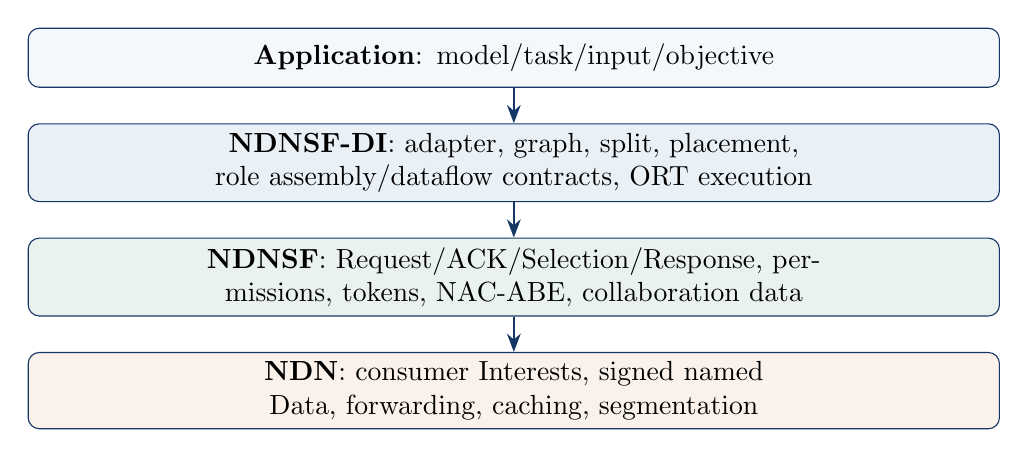
\begin{tikzpicture}[node distance=.45cm,
  box/.style={rounded corners,draw=Navy,text width=12.1cm,minimum height=.75cm,align=center},
  arr/.style={-{Stealth},thick,Navy}]
\node[box,fill=Light] (app) {\textbf{Application}: model/task/input/objective};
\node[box,fill=Blue!10,below=of app] (di) {\textbf{NDNSF-DI}: adapter, graph, split, placement, role assembly/dataflow contracts, ORT execution};
\node[box,fill=Green!10,below=of di] (core) {\textbf{NDNSF}: Request/ACK/Selection/Response, permissions, tokens, NAC-ABE, collaboration data};
\node[box,fill=Orange!10,below=of core] (ndn) {\textbf{NDN}: consumer Interests, signed named Data, forwarding, caching, segmentation};
\draw[arr] (app)--(di);\draw[arr] (di)--(core);\draw[arr] (core)--(ndn);
\end{tikzpicture}
\end{center}
\claim{Cross-Provider activations and tensor collectives remain NDN Interest/Data; ONNX Runtime performs only Provider-local compute.}
\end{frame}

\begin{frame}{Core Vocabulary and Immutable Identities}
\small
\begin{tabularx}{\textwidth}{>{\bfseries\raggedright\arraybackslash}p{3.4cm}>{\raggedright\arraybackslash}X}
\toprule
Invocation & One application-visible operation with one handle and terminal result.\\
Attempt & One bounded network decision generation inside an invocation.\\
ACK-closed snapshot & Immutable authenticated candidate set and its canonical digest.\\
Plan commit & One-shot generic projection of roles, dependencies, Providers, and opaque assignments.\\
Selection & ProviderToken-authorized final assignment sent to each chosen Provider.\\
Generation & Role execution epoch that fences late data and superseded work.\\
\bottomrule
\end{tabularx}
\claim{Identity and state transitions, not timing assumptions, determine which work is current.}
\nextline{start from the public application call}
\end{frame}

\begin{frame}{Single-Pass and Autoregressive Models Use Different Flows}
\scriptsize
\begin{columns}[T,onlytextwidth]
\column{.48\textwidth}
\textbf{Single-pass model (for example, YOLO)}
\begin{center}
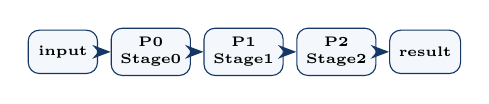
\begin{tikzpicture}[node distance=.16cm,
 b/.style={rounded corners,draw=Navy,fill=Light,minimum width=.88cm,minimum height=.55cm,align=center,font=\tiny\bfseries},
 a/.style={-{Stealth},thick,Navy}]
\node[b] (r) {input};
\node[b,right=of r] (p0) {P0\\Stage0};
\node[b,right=of p0] (p1) {P1\\Stage1};
\node[b,right=of p1] (p2) {P2\\Stage2};
\node[b,right=of p2] (o) {result};
\draw[a] (r)--(p0);\draw[a] (p0)--(p1);\draw[a] (p1)--(p2);\draw[a] (p2)--(o);
\end{tikzpicture}
\end{center}
\begin{itemize}
  \item One invocation moves from P0 to P2 once. P2 returns the final result.
  \item No output feeds back into another model pass.
\end{itemize}
\column{.50\textwidth}
\textbf{Autoregressive LLM generation}
\begin{center}
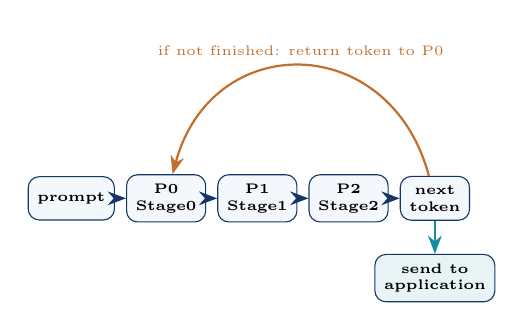
\begin{tikzpicture}[node distance=.14cm,
 b/.style={rounded corners,draw=Navy,fill=Light,minimum width=.88cm,minimum height=.55cm,align=center,font=\tiny\bfseries},
 a/.style={-{Stealth},thick,Navy},
 f/.style={-{Stealth},thick,Orange},
 e/.style={-{Stealth},thick,Cyan}]
\node[b] (r) {prompt};
\node[b,right=of r] (p0) {P0\\Stage0};
\node[b,right=of p0] (p1) {P1\\Stage1};
\node[b,right=of p1] (p2) {P2\\Stage2};
\node[b,right=of p2] (t) {next\\token};
\node[b,fill=Cyan!10,below=.42cm of t] (u) {send to\\application};
\draw[a] (r)--(p0);\draw[a] (p0)--(p1);\draw[a] (p1)--(p2);\draw[a] (p2)--(t);
\draw[e] (t)--(u);
\draw[f] (t) to[out=105,in=75,looseness=1.5]
  node[above,font=\tiny,align=center] {if not finished: return token to P0} (p0);
\end{tikzpicture}
\end{center}
\begin{itemize}
  \item Prefill sends the full prompt from P0 to P2 once.
  \item P2 publishes each new token to the application and feeds it back to P0. The token then passes through P0, P1, and P2 again.
\end{itemize}
\end{columns}
\vspace{-1.1em}
\claim{A single-pass invocation crosses the pipeline once. Autoregressive generation repeats the pipeline for each new token.}
\end{frame}

\input{prefill-decode-frames.tex}

\begin{frame}{Model Identity: Name Is Discovery, Digests Are Authority}
\begin{itemize}
  \item \textbf{model name}: readable discovery, logging, and operator policy;
  \item \textbf{content digest}: canonical signed manifest binding weights, graph, and configuration;
  \item \textbf{semantics digest}: tokenizer, preprocessing, generation defaults, output interpretation;
  \item \textbf{source revision}: provenance only; never substitutes for either digest.
\end{itemize}
\claim{Reuse requires exact content, semantics, graph, backend, precision, and runtime compatibility---not a matching model name.}
\nextline{make model-specific knowledge replaceable}
\end{frame}

\begin{frame}{One Carrier, Multiple Model Families}
\small
\begin{tabularx}{\textwidth}{>{\bfseries}p{2.5cm}X>{\raggedright\arraybackslash}p{3.6cm}}
\toprule
Adapter port & Responsibility & Forbidden authority\\
\midrule
Graph & canonical dependency snapshot & network or device mutation\\
Splitter & bounded graph-valid candidates & publication or Selection\\
Task & input/options/result schemas & placement or execution\\
State & lifecycle and exact state identity & cross-tenant access\\
Runner & execute accepted ONNX role & changing the plan or cross-Provider transport\\
\bottomrule
\end{tabularx}
\smallgap
The deployed runtime uses ONNX Runtime; PyTorch/Transformers are confined to a sealed offline exporter.
\claim{An opaque model may expose one atomic node; it remains runnable but is never falsely split.}
\nextline{derive placement structure from a real model graph}
\end{frame}

\begin{frame}{Dependency Graph: The Basis of a Legal Split}
\begin{columns}[T,onlytextwidth]
\column{.58\textwidth}
\begin{center}
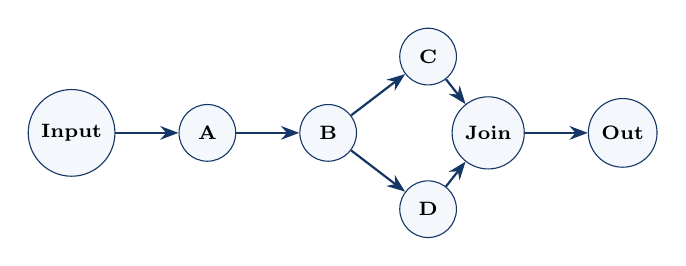
\begin{tikzpicture}[node distance=.8cm,
 n/.style={circle,draw=Navy,fill=Light,minimum size=.72cm,font=\scriptsize\bfseries},
 a/.style={-{Stealth},thick,Navy}]
\node[n] (i) {Input};
\node[n,right=of i] (a) {A};
\node[n,right=of a] (b) {B};
\node[n,above right=.45cm and .75cm of b] (c) {C};
\node[n,below right=.45cm and .75cm of b] (d) {D};
\node[n,right=1.2cm of b] (j) {Join};
\node[n,right=of j] (o) {Out};
\draw[a] (i)--(a);\draw[a] (a)--(b);\draw[a] (b)--(c);
\draw[a] (b)--(d);\draw[a] (c)--(j);\draw[a] (d)--(j);\draw[a] (j)--(o);
\end{tikzpicture}
\end{center}
\column{.40\textwidth}
\begin{itemize}
  \item nodes and topological order;
  \item tensor edges, dtype, shape, size estimate;
  \item legal cut edges and collective operations;
  \item model input/output contracts;
  \item canonical graph digest.
\end{itemize}
\end{columns}
\claim{Each tensor rank is a separate execution role assigned to exactly one Provider; the parallel group is metadata, not a cross-Provider role.}
\nextline{follow one invocation end to end}
\end{frame}

\begin{frame}{Complete Lifecycle: One Request, One Final Plan}
\scriptsize
\begin{center}
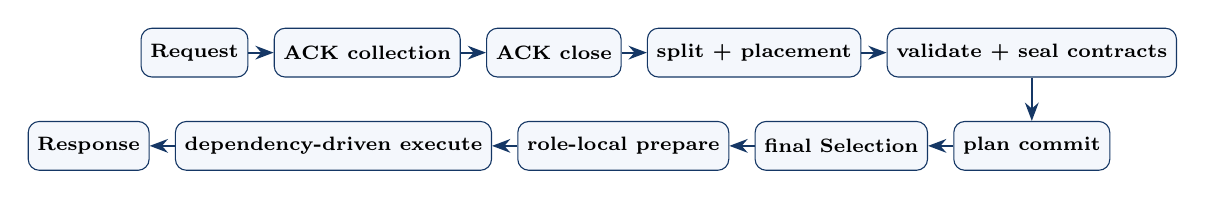
\begin{tikzpicture}[node distance=.32cm,
 b/.style={rounded corners,draw=Navy,fill=Light,minimum height=.62cm,align=center,font=\scriptsize\bfseries},
 a/.style={-{Stealth},thick,Navy}]
\node[b] (r) {Request};
\node[b,right=of r] (ack) {ACK collection};
\node[b,right=of ack] (close) {ACK close};
\node[b,right=of close] (plan) {split + placement};
\node[b,right=of plan] (mat) {validate + seal contracts};
\node[b,below=.55cm of mat] (commit) {plan commit};
\node[b,left=of commit] (sel) {final Selection};
\node[b,left=of sel] (prep) {role-local prepare};
\node[b,left=of prep] (exec) {dependency-driven execute};
\node[b,left=of exec] (resp) {Response};
\draw[a] (r)--(ack);\draw[a] (ack)--(close);\draw[a] (close)--(plan);\draw[a] (plan)--(mat);
\draw[a] (mat)--(commit);\draw[a] (commit)--(sel);\draw[a] (sel)--(prep);\draw[a] (prep)--(exec);\draw[a] (exec)--(resp);
\end{tikzpicture}
\end{center}
\begin{itemize}
  \item Positive ACK means willingness and bounded capability, not role acceptance or model readiness.
  \item After Selection, each Provider fetches canonical ONNX components and assembles one local role.
  \item A role issues Interests for its declared inputs and runs after all are verified.
\end{itemize}
\claim{No preparation-commit round and no global readiness barrier exist.}
\nextline{inspect the request and offer phases}
\end{frame}

\begin{frame}{Request Envelope: Signed Intent and Bounded Work}
\begin{itemize}
  \item binds invocation ID, request ID, attempt, service, model identity, task, input manifest;
  \item binds deadline, security domain, encoding version, capability version, and acceptance predicate;
  \item payloads are canonical, bounded, schema-identified bytes;
  \item UserToken and normal NDNSF authorization protect the wire request.
\end{itemize}
\claim{The request authorizes discovery for this exact operation; it does not authorize any Provider to execute.}
\nextline{define what a positive ACK can safely claim}
\end{frame}

\begin{frame}{Signed Provider Offer: Capability Without Role Commitment}
\small
\begin{columns}[T,onlytextwidth]
\column{.49\textwidth}
\textbf{Resource and network view}
\begin{itemize}
  \item Provider identity and boot epoch;
  \item one execution slot/device, backend, usable memory;
  \item queue depth and wait estimate;
  \item measured RTT and bandwidth;
  \item expiry, capture time, units, confidence.
\end{itemize}
\column{.49\textwidth}
\textbf{Reusable assets}
\begin{itemize}
  \item loaded role / assembled role / canonical component residency;
  \item lease/pin capability and generation;
  \item bounded reusable-state digests;
  \item artifact/runtime compatibility evidence.
\end{itemize}
\end{columns}
\claim{ACK evidence is fresh, signed, request-bound, and sanitized before policy code sees it.}
\nextline{freeze the candidate set before planning}
\end{frame}

\begin{frame}{ACK Closure: The Planning Linearization Point}
\begin{itemize}
  \item ACK collection closes exactly once at the discovery deadline.
  \item The ordered successful candidate set receives a canonical digest.
  \item Late ACKs cannot mutate the snapshot.
  \item Repeated reads return the same snapshot.
  \item Tokens, keys, leases, and mutable Core handles are removed from the policy view.
\end{itemize}
\claim{Every placement decision is reproducibly bound to one immutable ACK-closed digest.}
\nextline{invoke one narrow, replaceable planning extension}
\end{frame}

\begin{frame}[fragile]{Placement Extension: Pure Decision, No Side Effects}
\begin{lstlisting}[language=Python]
class ModelPlacementStrategy(ABC):
    name: str
    version: str
    state_digest: str
    @abstractmethod
    def plan(self, request: PlacementRequest) -> PlacementDecision:
        ...
\end{lstlisting}
\small
\begin{itemize}
  \item Input: model, graph, bounded candidates, sanitized Providers, network/catalog estimates, objective, and state contracts.
  \item Output: one certified split, one Provider per role, fallbacks, digests, and evidence.
  \item The implementation is local, allowlisted, digest-pinned operator-trusted code.
\end{itemize}
\claim{Policy output is revalidated as untrusted data; the Python interface is not a sandbox.}
\nextline{show the default policy}
\end{frame}

\begin{frame}{Default Policy: ACK-Driven PreSplitFirst}
\begin{enumerate}
  \item reject model, graph, backend, resource, freshness, and role mismatches;
  \item prefer an exact feasible certified split candidate;
  \item score loaded roles, assembled roles, canonical layers, network, and queue;
  \item otherwise derive a new graph-valid split from the closed offers;
  \item rank feasible bindings by predicted end-to-end critical-path cost;
  \item break ties with canonical digests for deterministic replay.
\end{enumerate}
\claim{PreSplitFirst remains the default; layer reuse is one cost signal, not a separate LayerReuseFirst architecture.}
\nextline{explain why byte size alone is unsafe}
\end{frame}

\begin{frame}{Capacity-Safe Splitting: Runtime Peak, Not File Size}
\[
M_{\mathrm{peak}} =
M_{\mathrm{weights}} + M_{\mathrm{activations}} + M_{\mathrm{state}} +
M_{\mathrm{workspace}} + M_{\mathrm{transient}} + M_{\mathrm{margin}}
\]
\begin{itemize}
  \item each role must fit the Provider's usable envelope;
  \item graph cuts must preserve dependency and tensor contracts;
  \item homogeneous stages use deterministic near-equal balancing only when safe;
  \item missing safe bounds yields \texttt{NO\_FEASIBLE\_SPLIT}, not optimistic admission.
\end{itemize}
\claim{``30 GB model / three 12 GB GPUs'' is not a valid memory proof.}
\nextline{turn cold-start cost into exact future reuse}
\end{frame}

\begin{frame}{Cache Residency: Evidence Has a Strength Order}
\begin{center}
\Large
\pill{Green}{LOADED ORT ROLE}
$>$ \pill{Cyan}{ASSEMBLED ROLE}
$>$ \pill{Blue}{CANONICAL LAYERS}
$>$ \pill{Orange}{REPOSITORY FETCH}
$>$ \pill{Red}{COLD ASSEMBLY}
\end{center}
\vspace{.8em}
\begin{itemize}
  \item Residency is Provider state, not a property of the catalog.
  \item Boot epoch, cache generation, expiry, identity, precision, and runtime ABI must match.
  \item Loaded-runtime identity also binds Provider boot/process/device and assembler/ORT ABI.
\end{itemize}
\claim{Warm reuse is an optimization guarded by exact evidence; clean loading remains the correctness fallback.}
\nextline{separate immutable artifacts from volatile residency}
\end{frame}

\begin{frame}{Pre-Split Catalog and Distributed Repository}
\small
\begin{columns}[T,onlytextwidth]
\column{.48\textwidth}
\textbf{Catalog owns}
\begin{itemize}
  \item canonical ONNX graph/initializer/tokenizer manifests;
  \item certified split candidates without Provider bindings;
  \item role/rank interfaces, collective DAG, size and backend contracts;
  \item activation, retirement, and revocation snapshots.
\end{itemize}
\column{.48\textwidth}
\textbf{Distributed repository owns}
\begin{itemize}
  \item signed named-object storage and retrieval;
  \item segmentation, checksums, replication evidence;
  \item deterministic canonical artifact Data names;
  \item Provider fetch before local ONNX assembly.
\end{itemize}
\end{columns}
\claim{Persistent model artifacts use the repository; request-scoped tensors use the producing Provider's namespace.}
\nextline{seal the validated decision into the generic collaboration}
\end{frame}

\begin{frame}{Plan Commit: Immutable Role and Dataflow Projection}
\begin{itemize}
  \item binds the exact ACK-closed digest;
  \item every role appears once; every Provider receives at most one role;
  \item each assignment binds one \texttt{RoleAssemblySpec};
  \item \texttt{mayPublish}, \texttt{mustFetch}, and \texttt{waitFor} form its \texttt{RoleDataflowContract};
  \item the first valid commit digest is immutable;
  \item failed validation emits zero Selection messages.
\end{itemize}
\claim{Plan commit is not Provider acceptance and does not consume a ProviderToken.}
\nextline{make each final Selection crash-atomic}
\end{frame}

\begin{frame}{Final Selection: Complete Role Authority}
\begin{itemize}
  \item exactly one complete execution role per selected Provider;
  \item rank, assembly recipe, canonical components, dependencies, budgets, generation;
  \item exact publish/fetch/wait name templates and collective rounds;
  \item protected by the selected Provider's one-time ProviderToken;
  \item Provider verifies request, attempt, plan, role, artifact, dataflow, and security bindings;
  \item GPU execution-slot admission occurs JIT, not during ACK.
\end{itemize}
\claim{Execution authority begins only after the exact Selection is durably accepted.}
\nextline{prepare each role independently}
\end{frame}

\begin{frame}{Role-Local Preparation: No Global Barrier}
\small
\begin{tabularx}{\textwidth}{>{\bfseries}p{3.4cm}>{\raggedright\arraybackslash}X}
\toprule
Latch & Meaning\\
\midrule
Selection accepted & exact role authority is durable\\
Local model ready & canonical components, RoleAssemblySpec, ORT ABI, JIT slot, and state verified\\
Direct inputs ready & every exact Interest target in \texttt{waitFor} verified\\
\bottomrule
\end{tabularx}
\smallgap
A role becomes runnable only when all three latches hold for the same attempt, plan, and generation.
\claim{Each Provider assembles one local ONNX role; consumers pull every cross-Provider input by Interest.}
\nextline{show the data-driven trigger}
\end{frame}

\begin{frame}{Data-Driven Execution: Consumer Pulls by Interest}
\[
\mathrm{Runnable}(r,g) =
\mathrm{Accepted}(r,g)\ \land\
\mathrm{LocalReady}(r,g)\ \land\
\bigwedge_{d\in\mathrm{DirectInputs}(r)}\mathrm{Verified}(d,g)
\]
\begin{itemize}
  \item \texttt{mayPublish}: exact output name templates owned by this role;
  \item \texttt{mustFetch}: exact Interests this role must express;
  \item \texttt{waitFor}: exact ALL/ANY/quorum readiness rule (collectives normally ALL);
  \item retransmission re-expresses the same name; stale attempt/plan/group data fails closed.
\end{itemize}
\claim{No hidden TCP/RPC push, shared file, or cross-Provider opaque NCCL path may replace this contract.}
\nextline{generalize beyond a linear pipeline}
\end{frame}

\begin{frame}{One Scheduler for Pipeline and Tensor Parallel}
\small
\begin{center}
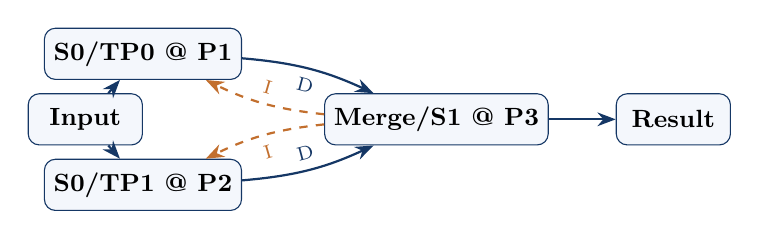
\begin{tikzpicture}[node distance=.85cm,
 n/.style={rounded corners,draw=Navy,fill=Light,minimum width=1.45cm,minimum height=.65cm,font=\small\bfseries},
 a/.style={-{Stealth},thick,Navy},
 interest/.style={-{Stealth},thick,dashed,Orange},
 data/.style={-{Stealth},thick,Navy}]
\node[n] (s0) {Input};
\node[n,right=of s0,above=.5cm] (s1) {S0/TP0 @ P1};
\node[n,right=of s0,below=.5cm] (s2) {S0/TP1 @ P2};
\node[n,right=2.3cm of s0] (j) {Merge/S1 @ P3};
\node[n,right=of j] (o) {Result};
\draw[a] (s0)--(s1);\draw[a] (s0)--(s2);
\draw[interest] (j) to[bend left=10] node[above,sloped,font=\scriptsize] {I} (s1);
\draw[data] (s1) to[bend left=10] node[below,sloped,font=\scriptsize] {D} (j);
\draw[interest] (j) to[bend right=10] node[below,sloped,font=\scriptsize] {I} (s2);
\draw[data] (s2) to[bend right=10] node[above,sloped,font=\scriptsize] {D} (j);
\draw[a] (j)--(o);
\end{tikzpicture}
\end{center}
\vspace{-.45em}
\begin{center}\scriptsize\color{Gray}
I = exact-name Interest issued by the consumer role; D = signed tensor Data returned by the producer role.
\end{center}
\vspace{-.35em}
\begin{itemize}
  \item each rank is a distinct role on one Provider;
  \item each round names producer, group/epoch, operation, rank, tensor, and segment;
  \item peers issue Interests for exact partials and advance only after the declared set arrives;
  \item missing rank, stale epoch, ambiguous producer, or unsatisfied join is rejected/fails closed.
\end{itemize}
\claim{A parallel group is metadata; if merge needs computation, merge is another execution role.}
\end{frame}

\begin{frame}{Intermediate Tensors: Deterministic NDN Names}
\scriptsize
\begin{block}{Producer-owned namespace}
\texttt{/<producer>/NDNSF/DI/TENSOR/<request>/<attempt>/<plan>/}\newline
\texttt{<group>/<epoch>/<op>/<round>/<src-role>/<tensor>/<microbatch>/<digest>/<segment>}
\end{block}
\begin{itemize}
  \item consumer first fetches a signed \texttt{TensorObjectManifest};
  \item manifest binds producer/consumer contract, dtype/shape/layout, segment count, and digests;
  \item consumer pipelines exact segment Interests and verifies before reassembly;
  \item duplicate/out-of-order Data is safe; wrong name, signer, digest, or epoch fails closed.
\end{itemize}
\claim{Request ID alone is insufficient: attempt, plan digest, group epoch, operation, rank, and segment prevent stale reuse.}
\nextline{define exactly one admissible final result}
\end{frame}

\begin{frame}{Result Contract: Events Are Not the Final Answer}
\begin{itemize}
  \item sealed before execution: terminal role(s), aggregation rule, output schema, acceptance predicate;
  \item binds model/task/input/plan/attempt identities and result digest;
  \item unary execution publishes no partial result and completes with one Response;
  \item streaming execution may publish ordered, attempt-bound Event Data, but no event is the terminal result;
  \item EOS, stop, token bound, cancellation, or failure produces a terminal stream state; Response is accepted only after the complete result passes the sealed contract.
\end{itemize}
\claim{Streaming changes when output becomes visible; it does not weaken the complete-result contract or the single terminal-Response invariant.}
\nextline{separate durable intent from bounded retransmission}
\end{frame}

\begin{frame}{One Plan Governs Each Generation Attempt}
\scriptsize
\begin{center}
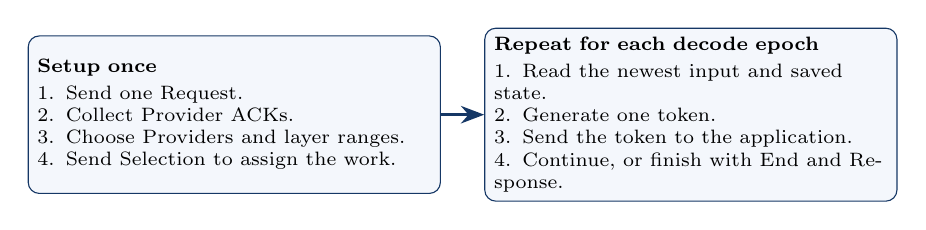
\begin{tikzpicture}[node distance=.55cm,
 b/.style={rounded corners,draw=Navy,fill=Light,text width=5.0cm,minimum height=2.0cm,align=left,font=\scriptsize},
 a/.style={-{Stealth},very thick,Navy}]
\node[b] (setup) {\textbf{Setup once}\\[.2em]
1. Send one Request.\\
2. Collect Provider ACKs.\\
3. Choose Providers and layer ranges.\\
4. Send Selection to assign the work.};
\node[b,right=of setup] (repeat) {\textbf{Repeat for each decode epoch}\\[.2em]
1. Read the newest input and saved state.\\
2. Generate one token.\\
3. Send the token to the application.\\
4. Continue, or finish with End and Response.};
\draw[a] (setup)--(repeat);
\end{tikzpicture}
\end{center}
\begin{itemize}
  \item One healthy attempt keeps the same request ID, accepted ACK set, and plan for the whole generation.
  \item Every Data name identifies the attempt, role, and decode epoch. Lost Data is requested again by the same exact name; late or wrong-step Data is rejected.
  \item A different Provider assignment creates one new attempt inside the same application invocation. At most one terminal result wins.
\end{itemize}
\claim{Discovery and placement happen once per attempt, not once per token. Recovery does not create a second application request.}
\nextline{compose independent state machines}
\end{frame}

\begin{frame}{Orthogonal State Machines, One Auditable History}
\scriptsize
\begin{tabularx}{\textwidth}{>{\bfseries}p{2.8cm}X}
\toprule
Machine & Principal states\\
\midrule
Invocation & open $\rightarrow$ terminal success / failure / cancelled / expired\\
Attempt & discovering $\rightarrow$ ACK closed $\rightarrow$ planned $\rightarrow$ executing $\rightarrow$ terminal\\
Plan commit & open $\rightarrow$ committing $\rightarrow$ committed or terminal failure\\
Provider transaction & none $\rightarrow$ prepared $\rightarrow$ applied $\rightarrow$ finalized / rolled back\\
Role & selected $\rightarrow$ preparing $\rightarrow$ ready $\rightarrow$ running $\rightarrow$ terminal\\
Interest/Object & expected $\rightarrow$ expressed/fetching $\rightarrow$ verified or rejected\\
Parallel group & planned $\rightarrow$ round $n$ $\rightarrow$ complete or epoch-failed\\
\bottomrule
\end{tabularx}
\claim{Every transition is monotonic, digest-bound, deadline-bound, and replay-safe.}
\nextline{classify failures by the authority that can react}
\end{frame}

\begin{frame}{Failure Taxonomy and Required Reaction}
\scriptsize
\begin{tabularx}{\textwidth}{>{\raggedright\arraybackslash\bfseries}p{3.3cm}X}
\toprule
Failure class & Required reaction\\
\midrule
Invalid offer, split, or policy output & exclude candidate; emit no Selection\\
Canonical fetch / local assembly failure & fail role/attempt; never emit partial downstream output\\
Selection delivery unknown & reconcile or retry identical protected bytes\\
Local load/state miss & use sealed clean-compute fallback or replan\\
Interest timeout/corruption/rank loss & fail affected role/group/attempt; fence the epoch\\
Provider crash/partition & fence generation; reconcile durable transaction\\
Result mismatch & reject Response; terminal failure or new attempt\\
\bottomrule
\end{tabularx}
\nextline{bound replanning and compensation}
\end{frame}

\begin{frame}{Replanning, Compensation, and Old-Output Adoption}
\begin{itemize}
  \item Replanning creates a new attempt with new assignment and generation identities.
  \item Old roles are cancelled or fenced; reservations and pins are released.
  \item Already published outputs are not silently reused.
  \item Adoption is allowed only if the new plan explicitly accepts the exact object contract and digest.
  \item Irreversible external side effects require application-level compensation.
\end{itemize}
\claim{Recovery never lets a late old output cross an attempt boundary by accident.}
\nextline{make cancellation and deadlines converge}
\end{frame}

\begin{frame}{Cancellation, Deadlines, and Resource Release}
\begin{itemize}
  \item one total invocation deadline continues through discovery, planning, fetch, assembly, loading, and execution;
  \item cancellation fences planner results, future commits, roles, objects, and Response;
  \item the first durable terminal state wins through compare-and-set;
  \item release covers execution-slot admission, cache pins, group keys, local assembly, tensor segments, and handles;
  \item unresolved delivery becomes explicit \texttt{UNKNOWN}, never implicit success.
\end{itemize}
\claim{Safety is preserved even when liveness is lost under a permanent partition.}
\nextline{trace the security chain}
\end{frame}

\begin{frame}{End-to-End Security Chain}
\footnotesize
\begin{enumerate}
  \item Controller-signed encrypted permissions authorize requester and Provider identities.
  \item NAC-ABE routes Request/Selection to service attributes and ACK/Response to permission attributes.
  \item UserToken binds ACK and Response to the request.
  \item one-time ProviderToken binds final Selection to the chosen Provider.
  \item a Provider-specific grant binds request, attempt, plan core, policy snapshot, and protection epoch.
  \item group capabilities disclose only the local wrapped epoch key; keys/nonces bind the exact role, peer, tensor manifest, and Data name.
  \item \texttt{ProtectedRuntime} rejects mismatches before ORT and zeroizes device then host plaintext on cancel/revoke.
\end{enumerate}
\claim{No planning optimization bypasses NDNSF authorization, token, signature, or replay controls.}
\nextline{limit what resource and cache evidence reveals}
\end{frame}

\begin{frame}{Privacy of Resource and Cache Metadata}
\begin{itemize}
  \item expose bounded summaries, not device handles or unrestricted inventories;
  \item publish digests, tier, bytes, freshness, and capability---not prompts, token IDs, plaintext state, or tenant names;
  \item retain raw tokens and keys only in protected runtime state;
  \item encrypt protected Selection retry material at rest and expire it;
  \item deny cross-tenant inference-state reuse by default.
\end{itemize}
\claim{The placement policy receives enough evidence to decide, but not enough authority to inspect or mutate Provider state.}
\nextline{quantify the model state kept by each Provider}
\end{frame}

\begin{frame}{Model-State Memory for One Context on Each Provider}
\scriptsize
\textbf{Qwen3.6-27B; fixed three-Provider split; batch size 1}
\par
\smallgap
{\footnotesize Context = prompt tokens + generated tokens still kept in memory.}
\smallgap
\begin{center}
\begin{tabular}{lccc}
\toprule
Provider and layers & 10K-token context & 100K-token context & 256K-token context\\
\midrule
P0: Stage0 $[0,21)$ & 245 MiB & 1.96 GiB & 5.05 GiB\\
P1: Stage1 $[21,42)$ & 245 MiB & 1.96 GiB & 5.05 GiB\\
P2: Stage2 $[42,64)$ & 284 MiB & 2.34 GiB & 6.05 GiB\\
\bottomrule
\end{tabular}
\end{center}
\vspace{.15em}
\begin{itemize}
  \item State grows with context: P0/P1 have 5 full-attention layers; P2 has 6.
  \item At 256K, FP16 weights plus state need about 22.3 GiB on P0, 19.9 GiB on P1, and 24.0 GiB on P2.
  \item A 32 GiB RTX 5000 Ada fits these static totals, but P2 leaves about 8 GiB for runtime memory. It is suitable for short-context validation; full 256K remains unverified.
\end{itemize}
{\tiny 256K means the native 262,144-token limit; the YaRN extension is not evaluated. Each concurrent sequence needs its own state.}

{\tiny\color{Gray}Estimate assumes batch size 1, FP16 KV/convolution state, FP32 recurrent state, and the shown 21/21/22-layer split.}
\nextline{explain why each Provider must keep saved state}
\end{frame}

\begin{frame}{Why Saved State Matters}
\scriptsize
\begin{columns}[T,onlytextwidth]
\column{.49\textwidth}
\begin{block}{Without saved state}
To generate token $n$, process the prompt and all earlier tokens again.
\end{block}
\begin{center}
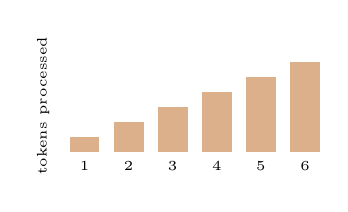
\begin{tikzpicture}[x=.56cm,y=.42cm]
\foreach \x/\h in {1/1,2/2,3/3,4/4,5/5,6/6}{
  \fill[Orange!55] (\x,0) rectangle +(0.68,\h/2.2);
  \node[font=\tiny,below] at (\x+.34,0) {\x};
}
\node[rotate=90,font=\tiny] at (.4,1.4) {tokens processed};
\end{tikzpicture}
\end{center}
Repeated work grows after every new token.
\column{.49\textwidth}
\begin{block}{With saved state}
Process the prompt once. Each later round uses one new token and the saved state.
\end{block}
\begin{center}
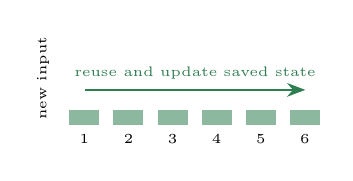
\begin{tikzpicture}[x=.56cm,y=.42cm]
\foreach \x in {1,...,6}{
  \fill[Green!55] (\x,0) rectangle +(0.68,.45);
  \node[font=\tiny,below] at (\x+.34,0) {\x};
}
\node[rotate=90,font=\tiny] at (.4,1.4) {new input};
\draw[-{Stealth},thick,Green] (1.35,1.05)--(6.35,1.05) node[midway,above,font=\tiny] {reuse and update saved state};
\end{tikzpicture}
\end{center}
Earlier tokens still affect the result through the saved state.
\end{columns}
\vspace{-.25em}
\begin{itemize}
  \item Each Provider keeps the attention KV, recurrent, and convolution state produced by its own layers.
  \item New state is committed only after the Provider successfully publishes its output; a failed step discards it.
\end{itemize}
\claim{Saved state avoids rebuilding earlier model state; it does not remove the LLM's dependence on earlier tokens.}
\nextline{show what moves between Providers and what stays local}
\end{frame}

\begin{frame}{What Moves Between Providers---and What Stays Local}
\scriptsize
\begin{center}
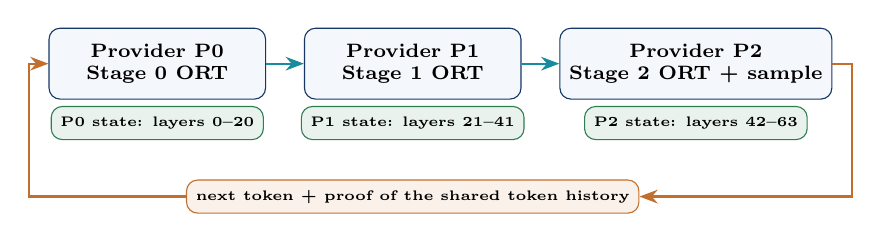
\begin{tikzpicture}[node distance=.48cm,
 p/.style={rounded corners,draw=Navy,fill=Light,minimum width=2.75cm,minimum height=.9cm,align=center,font=\scriptsize\bfseries},
 k/.style={rounded corners,draw=Green,fill=Green!10,minimum width=2.1cm,minimum height=.42cm,align=center,font=\tiny\bfseries},
 a/.style={-{Stealth},thick,Cyan},
 f/.style={-{Stealth},thick,Orange}]
\node[p] (p0) {Provider P0\\Stage 0 ORT};
\node[p,right=of p0] (p1) {Provider P1\\Stage 1 ORT};
\node[p,right=of p1] (p2) {Provider P2\\Stage 2 ORT + sample};
\node[k,below=.08cm of p0] (k0) {P0 state: layers 0--20};
\node[k,below=.08cm of p1] (k1) {P1 state: layers 21--41};
\node[k,below=.08cm of p2] (k2) {P2 state: layers 42--63};
\node[rounded corners,draw=Orange,fill=Orange!10,below=.5cm of k1,minimum width=4.2cm,minimum height=.42cm,font=\tiny\bfseries] (fb) {next token + proof of the shared token history};
\draw[a] (p0)--(p1);
\draw[a] (p1)--(p2);
\draw[f] (p2.east) -- ++(.25,0) |- (fb.east);
\draw[f] (fb.west) -| ([xshift=-.25cm]p0.west) -- (p0.west);
\end{tikzpicture}
\end{center}
\begin{itemize}
  \item Each Provider keeps the state produced by its own model layers. These three states are different and cannot replace one another.
  \item All roles verify the same token-history digest, token count, and next position. Their local state tensors remain different.
  \item NDN carries authenticated activation and token-feedback Data. It does not carry the large saved-state tensors.
  \item P2 publishes the external token Event and the internal feedback Data separately.
\end{itemize}
\claim{A shared proof of token history keeps three different Provider states synchronized without transferring those states over NDN.}
\nextline{show when saved state is safe to reuse}
\end{frame}

\begin{frame}{When Saved State Can Be Reused Safely}
\scriptsize
\begin{columns}[T,onlytextwidth]
\column{.45\textwidth}
\textbf{Reuse state only when all conditions match}
\begin{itemize}
  \item model artifact and tensor layout;
  \item Provider process and assigned layers;
  \item runtime and security context;
  \item request attempt and token prefix;
  \item exact previous decode epoch.
\end{itemize}
\column{.53\textwidth}
\textbf{One safe token-generation step}
\begin{center}
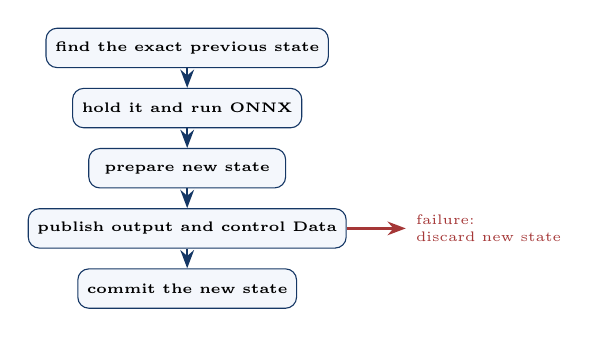
\begin{tikzpicture}[node distance=.25cm,
 b/.style={rounded corners,draw=Navy,fill=Light,minimum width=2.5cm,minimum height=.5cm,align=center,font=\tiny\bfseries},
 a/.style={-{Stealth},thick,Navy}]
\node[b] (l) {find the exact previous state};
\node[b,below=of l] (p) {hold it and run ONNX};
\node[b,below=of p] (s) {prepare new state};
\node[b,below=of s] (o) {publish output and control Data};
\node[b,below=of o] (c) {commit the new state};
\draw[a] (l)--(p);\draw[a] (p)--(s);\draw[a] (s)--(o);\draw[a] (o)--(c);
\draw[-{Stealth},thick,Red] (o.east) -- ++(.75,0) node[right,font=\tiny,align=left] {failure:\\discard new state};
\end{tikzpicture}
\end{center}
\end{columns}
\claim{A failed step discards its new state. Completion, cancellation, deadline, or Provider restart makes old request state unusable and removes it.}
\nextline{separate perceived latency from decode throughput}
\end{frame}

\begin{frame}{Continuous Generation: Optimize TTFT and TPOT}
\scriptsize
\begin{columns}[T,onlytextwidth]
\column{.47\textwidth}
\textbf{Critical-path metrics}
\smallgap

\textbf{TTFT} $=$ discovery + planning + role preparation + prefill + first Event Data

\smallgap
\textbf{TPOT} $\approx$ stage ORT + activation Interest/Data + sampling + feedback Interest/Data

\smallgap
\centering
\pill{Orange}{20 token/s target $\Rightarrow$ TPOT $\leq 50$ ms}
\column{.51\textwidth}
\textbf{Optimization order}
\begin{enumerate}
  \item keep ORT sessions, device buffers, and I/O bindings resident;
  \item prefill once; decode one token with the exact local saved state;
  \item pre-express exact activation, feedback, and Event Interests;
  \item sign/publish through a bounded asynchronous queue with backpressure;
  \item grant one stream content key, then protect events symmetrically---no per-token ABE bootstrap.
\end{enumerate}
\end{columns}
\claim{Streaming improves perceived latency; only incremental stateful decode and a shorter per-epoch path improve tokens/s. This is a target, not current performance evidence.}
\end{frame}

\begin{frame}{Observability: Evidence for Decisions and Execution}
\begin{itemize}
  \item planning input digest, strategy identity, candidate rejection reasons, selected cost components;
  \item ACK closure, plan commit, Selection transaction, role readiness, object verification, and terminal status;
  \item canonical fetch, local assembly, ORT load, Interest wait/retransmit, collective rounds, compute, TTFT, latency, tokens/s;
  \item sampled request-correlated traces with no plaintext prompt or secret material;
  \item \texttt{report\_operation\_status()} reports authenticated progress, not execution authority.
\end{itemize}
\nextline{show the implemented generic carrier calls}
\end{frame}

\begin{frame}[fragile]{Operator Configuration: Policy, Not Deployment}
\begin{lstlisting}
schema: ndnsf-di-application/v2
identity:
  requester: /ndnsf/di/user
  controller: /ndnsf/controller
repository:
  prefix: /ndnsf/di/models
planning:
  strategy: {name: pre-split-first, version: "3",
             digest: "sha256:<strategy-code-and-state>"}
  gpu_safety_margin: 0.15
cache:
  canonical_onnx_components: {retain_verified: true}
  derived_state:
    exact_prefix_local_reuse: true
    cross_tenant_reuse: false
    migration: disabled
\end{lstlisting}
\small No model, Provider list, role graph, private key, or precomputed deployment belongs here.
\nextline{map the design to current code}
\end{frame}

\begin{frame}{Implemented Surface and Current Qualification Boundary}
\scriptsize
\begin{tabularx}{\textwidth}{>{\bfseries}p{3.4cm}>{\raggedright\arraybackslash}X}
\toprule
Area & Current mechanism or explicit target boundary\\
\midrule
Generic carrier & deferred begin, immutable ACK closure, one-shot plan commit\\
Planning & common graph/candidate values, read-only catalog snapshot, external allowlist, default pre-split-first policy\\
Adapters & composed graph/split/task/state/runner ports with digest pins\\
Artifacts & canonical ONNX graph/initializer manifests; repository store/fetch; Provider-local assembly\\
Execution & one role per Provider; Interest pull; manifest/segment and collective-round gates\\
State & exact prefix-and-epoch identity, local reuse binding, clean-compute/replan fallback\\
Delivery & unary terminal Response and request-scoped ordered Event Data plus one terminal Response are implemented\\
Recovery/security & durable selection transaction, generations, cancellation, tokens, NAC-ABE\\
\bottomrule
\end{tabularx}
\claim{Multi-role Provider, cross-Provider logical role, DEVICE\_SET, and LayerReuseFirst-default paths are migration drift, not target completion evidence.}
\end{frame}

\begin{frame}{Validation Pyramid: Cheapest Correct Gate First}
\begin{enumerate}
  \item pure contract and negative unit tests;
  \item native build and binding checks;
  \item one-container security/control smoke with tiny payload;
  \item exact-SIF CPU small-ONNX pipeline/tensor/hybrid Interest/Data flows;
  \item MiniNDN multi-Provider lifecycle, negative names/epochs, then Qwen complete answers;
  \item optional Slurm/Apptainer network, CUDA, stage, and campaign gates.
\end{enumerate}
\claim{A higher-cost test does not repair a failed lower gate, and a lower gate does not prove a higher-layer claim.}
\nextline{report the accepted local evidence}
\end{frame}

\begin{frame}{CPU Check: Reuse State Instead of Reprocessing Old Tokens}
\small
\begin{center}
\textbf{Fixture: 1-token input context (token \texttt{3}) $\rightarrow$ 8 generated tokens.}\\
Both paths generated \texttt{4, 5, 6, 7, 8, 9, 10, 2}.
\end{center}
\smallgap
\begin{columns}[T,onlytextwidth]
\column{.48\textwidth}
\begin{block}{Reuse saved state}
Prefill reads the 1-token prompt; seven decode rounds each read one new token.\\[.5em]
\centering\large
$1+(7\times1)=\mathbf{8}$
\end{block}
\column{.48\textwidth}
\begin{alertblock}{Recompute the full history}
The complete prefix grows from 1 to 8 tokens.\\[.5em]
\centering\large
$1+2+3+4+5+6+7+8=\mathbf{36}$
\end{alertblock}
\end{columns}
\vspace{.35em}
\claim{For this 1-token context, saved state avoided 28 repeated token-position computations: $36-8=28$.}
\vspace{.25em}
{\footnotesize This is a correctness check with a tiny CPU ONNX model. It does not measure speed, GPU memory, or Qwen3.6-27B throughput.}
\nextline{separate verified behavior from remaining deployment work}
\end{frame}

\begin{frame}{Current Evidence Boundary}
\scriptsize
\begin{block}{Verified with the tiny CPU ONNX model}
\begin{itemize}
  \item one Request and plan produce ordered token Events, End, and one final Response;
  \item focused one-, two-, and four-Provider flows cover cancellation, deadline, tamper/replay rejection, and cleanup;
  \item Provider-owned state produces the same output as full-prefix recomputation while avoiding 28 prior-token positions.
\end{itemize}
\end{block}
\begin{alertblock}{Not yet verified}
\begin{itemize}
  \item GPU-resident KV/model state: the current ORT path still copies saved state into CPU buffers;
  \item a real Python application running across separate processes;
  \item Qwen3.6-27B GPU correctness, memory use, latency, and throughput.
\end{itemize}
\end{alertblock}
\vspace{-.55em}
\begin{center}
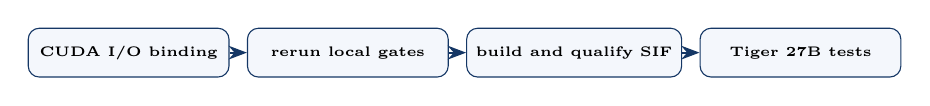
\begin{tikzpicture}[node distance=.22cm,
 s/.style={rounded corners,draw=Navy,fill=Light,minimum width=2.55cm,minimum height=.62cm,align=center,font=\tiny\bfseries},
 a/.style={-{Stealth},thick,Navy}]
\node[s] (a) {CUDA I/O binding};
\node[s,right=of a] (b) {rerun local gates};
\node[s,right=of b] (c) {build and qualify SIF};
\node[s,right=of c] (d) {Tiger 27B tests};
\draw[a] (a)--(b); \draw[a] (b)--(c); \draw[a] (c)--(d);
\end{tikzpicture}
\end{center}
\vspace{-.35em}
\claim{CPU tests validate semantics; GPU tests must validate device residency and performance.}
\end{frame}

\begin{frame}{Remaining Physical Requalification Boundary}
\begin{itemize}
  \item exact locally qualified SIF digest;
  \item actual allocated GPU model, UUID, memory, CUDA provider, and \texttt{cpuFallback=0};
  \item allocation-scoped cross-node NFD connectivity;
  \item role assembly hashes, complete graph/initializer coverage, and tensor-edge receipts;
  \item exact standalone reference tokens and full distributed answers;
  \item warmup-separated TTFT, per-token latency, total latency, and tokens/s distributions.
\end{itemize}
\claim{These are test-environment facts, not missing semantics in the NDNSF-DI lifecycle.}
\nextline{build the local container safely}
\end{frame}

\begin{frame}{Local SIF Step 1: Build Inside the Target ABI}
\begin{itemize}
  \item The release candidate begins as one complete locally built Apptainer SIF.
  \item Build native Python/C++ extensions inside that SIF or an ABI-identical sealed builder.
  \item Record source seal, base digest, Apptainer, Python SOABI, glibc, Boost, ndn-cxx, NDN-SVS, ORT/CUDA, and SIF SHA-256.
  \item Never copy a host-built \texttt{\_ndnsf.so} into the candidate.
  \item Keep models, NDN keys, credentials, and evidence outside the SIF.
\end{itemize}
\claim{The deployment SIF contains ONNX Runtime, not PyTorch/Transformers; those belong only in the offline exporter.}
\nextline{qualify the exact local candidate}
\end{frame}

\begin{frame}{Local SIF Step 2: Qualify the Exact Candidate}
\begin{itemize}
  \item Import \texttt{ndnsf.\_ndnsf}; run the real MiniNDN runner \texttt{--help}.
  \item Verify extension/native hashes, RPATH/\texttt{ldd} closure, SOABI, library versions, ORT providers, and absolute artifact paths.
  \item Run CPU small-ONNX Request/ACK/Selection and Provider-local assembly.
  \item Run pipeline and two-rank tensor Interest/Data flows plus negative name/epoch/rank tests.
  \item Reject stale extensions, host-library leakage, unresolved symbols, and cwd-dependent artifacts.
\end{itemize}
\claim{Host tests or a different SIF cannot qualify the file that will run on Tiger.}
\nextline{discover live cluster facts before upload}
\end{frame}

\begin{frame}[fragile]{iTiger Step 1: Read-Only Preflight}
\begin{lstlisting}
uofm-vpn-status
ssh -o BatchMode=yes itiger 'hostname; whoami'

tools/ndnsf-di/ndnsf-di-itiger-qwen discover --help
\end{lstlisting}
\begin{itemize}
  \item Recheck quota, partition, GRES spelling, Apptainer, driver, addresses, and scratch.
  \item Keep durable releases/models/evidence under \texttt{/project/\$USER/ndnsf-di}.
  \item Never build, convert, download a large model, or infer on the login node.
\end{itemize}
\nextline{upload the already-qualified immutable SIF}
\end{frame}

\begin{frame}{iTiger Step 2: Hash-Promote the Local SIF}
\begin{enumerate}
  \item Upload the locally qualified SIF to project staging; do not rebuild/materialize another candidate on Tiger.
  \item Verify source seal, manifest, and SIF SHA-256; atomically promote the exact file.
  \item Preflight sbatch: absolute SIF/bundle/model/evidence paths, cwd, binds, partition/GRES, Provider identities, and output directory.
  \item In a GPU allocation, run \texttt{apptainer exec --nv}; verify device, driver, ONNX Runtime CUDA, NFD, and NDNSF imports.
  \item Assert PyTorch/Transformers are absent and CPU fallback is disabled.
\end{enumerate}
\claim{Host PASS, exact local-SIF PASS, and Tiger GPU PASS are separate gates bound to one SIF hash.}
\nextline{advance through the Qwen test ladder}
\end{frame}

\begin{frame}{iTiger Step 3: Network, Reference, Stages, Then DI}
\begin{enumerate}
  \item \textbf{multi-node NFD probe}: no model; prove job-scoped faces and signed Data exchange;
  \item \textbf{standalone reference}: canonical ONNX, tokenizer, prompt set, greedy outputs;
  \item \textbf{role load}: one Provider per role, exact graph/initializer coverage, ORT CUDA, no CPU fallback;
  \item \textbf{full development invocation}: request/attempt/plan/group, assembly, Interest/Data edge and collective receipts, complete answer;
  \item \textbf{formal campaign}: frozen SIF/model/strategy/Provider count; warmup-separated repetitions.
\end{enumerate}
\claim{Run stages in this order; stop at the first failed gate and preserve it.}
\nextline{retain evidence and enforce stop rules}
\end{frame}

\begin{frame}{iTiger Step 4: Evidence, Distribution, and Stop Rules}
\begin{itemize}
  \item bind model/tokenizer, source, exact SIF digest, plan/group, role map, GPU UUIDs, job/run/repetition IDs;
  \item retain full answers, tokens, EOS, TTFT, latency, tokens/s, assembly, Interest wait/retransmit, collective and transfer timing;
  \item retain failed, timed-out, cancelled, mismatched, and truncated repetitions; exclude them from success summaries without deleting them;
  \item never silently retry a measured identity, change GPU count/type, quantize, extend time, or overwrite a failure;
  \item promote evidence before allocation scratch is removed.
\end{itemize}
\claim{One warm run is an anecdote; the frozen repeated campaign is the distribution.}
\nextline{close with the governing design principle}
\end{frame}

\begin{frame}{Persistent Artifacts vs. Request-Scoped Tensors}
\footnotesize
\begin{itemize}
  \item DistributedRepo owns persistent canonical ONNX graph/initializer/tokenizer objects: queued store, manifest trust, segmented Data, receipts, activation, recovery, and GC.
  \item Request-scoped activations and collective partials are published under the producing Provider's namespace and pulled directly by exact Interests.
  \item Both paths use signed segmented NDN Data, but their names, deadlines, authorization, freshness, and retention differ.
  \item Repo success does not prove pipeline/tensor dataflow; the corrected protocol needs its own exact-SIF and MiniNDN gates.
\end{itemize}
\begin{block}{Required separation}
Model artifacts are durable and content-addressed. Intermediate tensors are attempt/plan/group-epoch bound, short-lived, and accepted only by roles whose sealed \texttt{mustFetch}/\texttt{waitFor} contracts name them.
\end{block}
\nextline{close the corrected protocol before large-model performance claims}
\end{frame}

\begin{frame}{How the Complete Request Runs}
\begin{center}
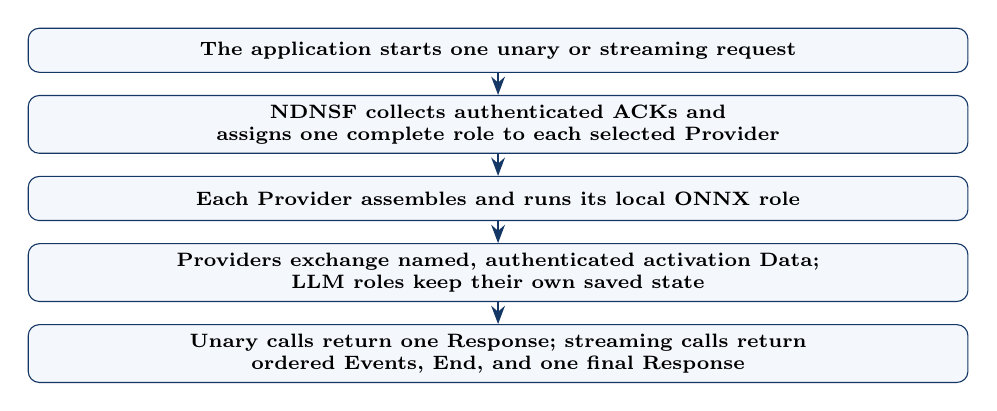
\begin{tikzpicture}[node distance=.28cm,
 b/.style={rounded corners,draw=Navy,fill=Light,text width=11.7cm,minimum height=.56cm,align=center,font=\scriptsize\bfseries},
 a/.style={-{Stealth},thick,Navy}]
\node[b] (a) {The application starts one unary or streaming request};
\node[b,below=of a] (b) {NDNSF collects authenticated ACKs and\\assigns one complete role to each selected Provider};
\node[b,below=of b] (c) {Each Provider assembles and runs its local ONNX role};
\node[b,below=of c] (d) {Providers exchange named, authenticated activation Data;\\LLM roles keep their own saved state};
\node[b,below=of d] (e) {Unary calls return one Response; streaming calls return\\ordered Events, End, and one final Response};
\draw[a] (a)--(b);\draw[a] (b)--(c);\draw[a] (c)--(d);\draw[a] (d)--(e);
\end{tikzpicture}
\end{center}
\vspace{.15em}
\begin{center}
\color{Navy}\large\bfseries One request. One plan per attempt.\\
ONNX state stays local; exact NDN Data moves between roles.
\end{center}
\end{frame}

\input{kv-cache-tiering-discussion.tex}

\end{document}
